%!TEX root = ./template-skripsi.tex
%-------------------------------------------------------------------------------
%                            BAB III
%               			PEMBAHASAN
%-------------------------------------------------------------------------------

\chapter{METODOLOGI PENELITIAN}

\section{Keterhubungan Penelitian}

\begin{figure}[H]
	\centering
	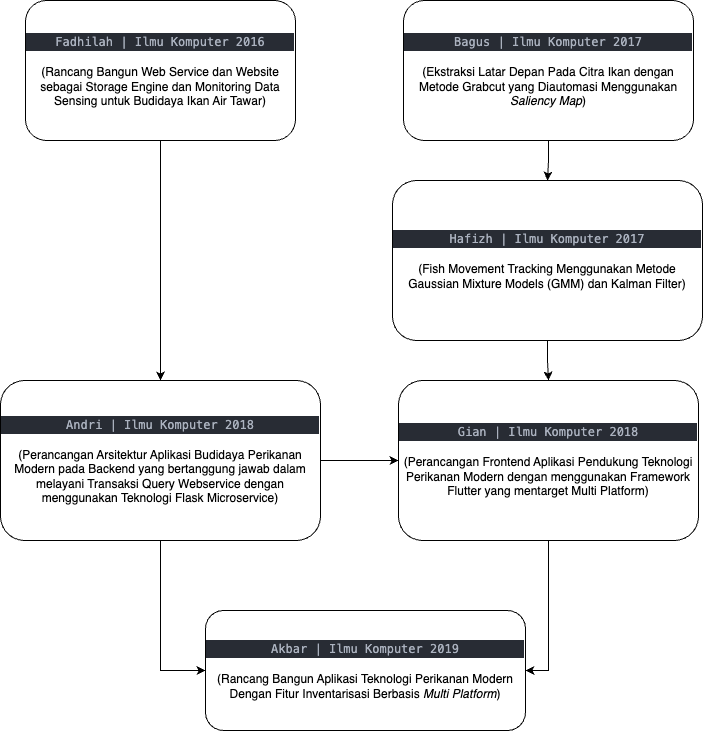
\includegraphics[width=0.7\textwidth]{gambar/akbar/research_tree.png}
	\caption{Diagram Alur Penelitian \textit{Aquaculture}}
\end{figure}

Pada diagram diatas, dapat dilihat urutan arah dari topik penelitian Aquaculture. Penelitian pertama kali dimulai oleh \citep{fadhil2022} dengan mengembangkan sebuah web service serta website yang berfungsi sebagai Storage Engine dan Monitoring Data Sensing untuk digunakan pada Budidaya Perikanan Air Tawar sebagai media penyimpanan data-data sensing dari sensor yang dikirimkan ke sistem serta memonitoringnya dalam bentuk table dan grafik real-time. 

Kemudian penelitian dilanjutkan oleh \citep{andri2022} dengan membuat ... yang dibarengi oleh penelitian \citep{gian2022} dari sisi mobile dalam pembuatan \dots

Pada topik penelitian Aquaculture, terdapat penelitian yang terkait tentang deteksi ikan. Penelitian tersebut dilakukan oleh ... yang berjudul ... dan ... yang berjudul ...

Dalam penelitian yang sudah berjalan ini, 

\section{Metode Penentuan Nilai Jual}

Dalam menentukan nilai jual, dapat digunakan rumus dibawah ini.

\section{Analisa Arsitektur Fitur}

Pada penelitian aplikasi yang sudah dikembangkan sebelumnya, terdapat use case yang menjelaskan konsep dari aplikasi yang ada pada gambar dibawah ini.


\section{Analisa Pengembangan Fitur}

Pada analisa arsitektur fitur yang ada di aplikasi sebelumnya, dapat dilengkapi dengan fitur inventaris yang akan dilakukan pada penelitian ini. Fitur tersebut memiliki use case diagram seperti berikut.

% \section{Stories}

%     \subsection{Pencatatan Inventaris}

%     \begin{enumerate}
%         \item Bahan baku
%         \begin{enumerate}
%             \item Pakan
%             \item Bahan organik
%         \end{enumerate}
%         \item Listrik
%         \item Benih
%     \end{enumerate}

%     \subsection{Depresiasi Aset}

%     \begin{enumerate}
%         \item Kadaluarsa bahan baku
%         \item Penurunan kualitas
%     \end{enumerate}